\documentclass{article}

\usepackage{amsmath,amsfonts,amsthm,latexsym,amssymb,amstext,mathabx,epic}
\usepackage[T1]{fontenc}
\usepackage[utf8]{inputenc}
\usepackage{karnaugh-map}
\usepackage{tikz}
\usepackage{bm}
\usepackage{mathtools}
\usepackage{makecell}
\usepackage{xcolor}
\usepackage{multicol}
\usepackage[absolute,overlay]{textpos}
\usepackage{graphicx}

\definecolor{_red}{RGB}      {252,192,194}
\definecolor{_blue}{RGB}     {190,193,247}
\definecolor{_lightBlue}{RGB}{191,230,244}
\definecolor{_green}{RGB}    {190,251,191}
\definecolor{_yellow}{RGB}   {253,252,183}
\definecolor{_purple}{RGB}   {245,195,222}

\newcommand{\highlightred}[1]{\colorbox   {_red}{$\displaystyle#1$}}
\newcommand{\highlightblue}[1]{\colorbox  {_blue}{$\displaystyle#1$}}
\newcommand{\highlightlblue}[1]{\colorbox {_lightBlue}{$\displaystyle#1$}}
\newcommand{\highlightpurple}[1]{\colorbox{_purple}{$\displaystyle#1$}}
\newcommand{\highlightyellow}[1]{\colorbox{_yellow}{$\displaystyle#1$}}
\newcommand{\highlightgreen}[1]{\colorbox {_green}{$\displaystyle#1$}}

\setcellgapes{1.5pt}

\usetikzlibrary{arrows,shapes.gates.logic.US,shapes.gates.logic.IEC,calc}
\tikzstyle{branch}=[fill,shape=circle,minimum size=3pt,inner sep=0pt]

\def\checkmark{\tikz\fill[scale=0.4](0,.35) -- (.25,0) -- (1,.7) -- (.25,.15) -- cycle;}
\newcommand*{\oline}[1]{\overline{#1\mathstrut}}
\newcommand{\bigspace}{\quad\quad\quad\quad}

\begin{document}
\author{Francesco Andreuzzi}
\title{Progetto - Fondamenti di informatica\\ \large{N. Matricola: IN0500630}}
\date{Anno 2018-2019}
\maketitle

\section{Calcolo della funzione}

\begin{textblock*}{10pt}(100pt,450pt)
  \begin{gather*}
    (500630 \mod \quad 65536) = 41878\\
    41878_{10} = 1010001110010110_2
  \end{gather*}
\end{textblock*}

\begin{textblock*}{10pt}(230pt,467pt)
  \Huge{\boldmath{$\implies$}}
\end{textblock*}

\begin{textblock*}{10pt}(300pt,360pt)
  \begin{tabular}{|c|c|c|c|c|}
    \hline
    \textbf{x} & \textbf{y} & \textbf{z} & \textbf{k} & \textbf{f(x,y,z,k)} \\
    \hline
      0 & 0 & 0 & 0 & 1 \\
    \hline
      0 & 0 & 0 & 1 & 0 \\
    \hline
      0 & 0 & 1 & 0 & 1 \\
    \hline
      0 & 0 & 1 & 1 & 0 \\
    \hline
      0 & 1 & 0 & 0 & 0 \\
    \hline
      0 & 1 & 0 & 1 & 0 \\
    \hline
      0 & 1 & 1 & 0 & 1 \\
    \hline
      0 & 1 & 1 & 1 & 1 \\
    \hline
      1 & 0 & 0 & 0 & 1 \\
    \hline
      1 & 0 & 0 & 1 & 0 \\
    \hline
      1 & 0 & 1 & 0 & 0 \\
    \hline
      1 & 0 & 1 & 1 & 1 \\
    \hline
      1 & 1 & 0 & 0 & 0 \\
    \hline
      1 & 1 & 0 & 1 & 1 \\
    \hline
      1 & 1 & 1 & 0 & 1 \\
    \hline
      1 & 1 & 1 & 1 & 0 \\
    \hline
  \end{tabular}
\end{textblock*}

Ricavo la funzione dal resto della divisione del numero di matricola per $2^{16}$:\\

\newpage

\subsection*{Minterm}
Riscrivo le combinazioni $(x,y,z,k)$ in cui la funzione assume valore $1$:\\
\begin{center}
  \begin{tabular}{|c|c|c|c|c|}
    \hline
    \textbf{x} & \textbf{y} & \textbf{z} & \textbf{k} & \textbf{f(x,y,z,k)} \\
    \hline
      0 & 0 & 0 & 0 & 1 \\
    \hline
      0 & 0 & 1 & 0 & 1 \\
    \hline
      0 & 1 & 1 & 0 & 1 \\
    \hline
      0 & 1 & 1 & 1 & 1 \\
    \hline
      1 & 0 & 0 & 0 & 1 \\
    \hline
      1 & 0 & 1 & 1 & 1 \\
    \hline
      1 & 1 & 0 & 1 & 1 \\
    \hline
      1 & 1 & 1 & 0 & 1 \\
    \hline
  \end{tabular}
\end{center}
La funzione $f(x,y,z,k)$ quindi si può esprimere nel seguente modo:
\begin{align*}
  \bm{f(x,y,z,k)} = (\oline{x} \cdot \oline{y} \cdot \oline{z} \cdot \oline{k}) + (\oline{x} \cdot \oline{y}\cdot z \cdot \oline{k})
      + (\oline{x} \cdot y \cdot z \cdot \oline{k}) + (\oline{x} \cdot y \cdot z \cdot k) + (x \cdot \oline{y} \cdot \oline{z} \cdot \oline{k})
        + (x \cdot \oline{y} \cdot z \cdot k) + \\ + (x \cdot y \cdot \oline{z} \cdot k) + (x \cdot y \cdot z \cdot \oline{k})
\end{align*}

\subsection*{Maxterm}
Riscrivo le combinazioni $(x,y,z,k)$ in cui la funzione assume valore $0$:
\begin{center}
  \begin{tabular}{|c|c|c|c|c|}
    \hline
    \textbf{x} & \textbf{y} & \textbf{z} & \textbf{k} & \textbf{f(x,y,z,k)} \\
    \hline
      0 & 0 & 0 & 1 & 0 \\
    \hline
      0 & 0 & 1 & 1 & 0 \\
    \hline
      0 & 1 & 0 & 0 & 0 \\
    \hline
      0 & 1 & 0 & 1 & 0 \\
    \hline
      1 & 0 & 0 & 1 & 0 \\
    \hline
      1 & 0 & 1 & 0 & 0 \\
    \hline
      1 & 1 & 0 & 0 & 0 \\
    \hline
      1 & 1 & 1 & 1 & 0 \\
    \hline
  \end{tabular}
\end{center}
La funzione $f(x,y,z,k)$ quindi si può esprimere nel seguente modo:
\begin{align*}
  \bm{f(x,y,z,k)} = (x+y+z+\oline{k}) \cdot (x+y+\oline{z}+\oline{k}) \cdot (x+\oline{y}+z+k) \cdot (x+\oline{y}+z+\oline{k}) \cdot (\oline{x}+y+z+\oline{k}) \cdot\\
  \cdot (\oline{x}+y+\oline{z}+k) \cdot (\oline{x}+\oline{y}+z+k) \cdot (\oline{x}+\oline{y}+\oline{z}+\oline{k})
\end{align*}

\section{Semplificazione}

\subsection*{Semplificazione algebrica}

\subsubsection*{Minterm}
\begin{align*}
  % line 1
  \bm{f(x,y,z,k)} &= \underline{(\oline{x} \cdot \oline{y} \cdot \oline{z} \cdot \oline{k})} + (\oline{x} \cdot \oline{y} \cdot z \cdot \oline{k}) + (\oline{x} \cdot y \cdot z \cdot \oline{k}) + (\oline{x} \cdot y \cdot z \cdot k) + \underline{(x \cdot \oline{y} \cdot \oline{z} \cdot \oline{k})} + (x \cdot \oline{y} \cdot z \cdot k) + \\
  &\bigspace + (x \cdot y \cdot \oline{z} \cdot k) + (x \cdot y \cdot z \cdot \oline{k})\\
  % line 2
  &\overset{T9}{=} (\oline{y} \cdot \oline{z} \cdot \oline{k}) + (\oline{x} \cdot \oline{y} \cdot z \cdot \oline{k}) + (\oline{x} \cdot y \cdot z \cdot \oline{k}) + (\oline{x} \cdot y \cdot z \cdot k) + (x \cdot \oline{y} \cdot z \cdot k) + (x \cdot y \cdot \oline{z} \cdot k)\\
  &\bigspace + (x \cdot y \cdot z \cdot \oline{k})\\
  % line 3
  &= (\oline{y} \cdot \oline{z} \cdot \oline{k}) + (\oline{x} \cdot \oline{y} \cdot z \cdot \oline{k}) + (\oline{x} \cdot y \cdot z \cdot \oline{k}) + (\oline{x} \cdot y \cdot z \cdot \oline{k}) + (\oline{x} \cdot y \cdot z \cdot \oline{k}) + (\oline{x} \cdot y \cdot z \cdot k) + \\
  &\bigspace + (x \cdot \oline{y} \cdot z \cdot k) + (x \cdot y \cdot \oline{z} \cdot k) + (x \cdot y \cdot z \cdot \oline{k})\\
  % line 4
  &= (\oline{y} \cdot \oline{z} \cdot \oline{k}) + \underline{(\oline{x} \cdot \oline{y} \cdot z \cdot \oline{k})} + \underline{(\oline{x} \cdot y \cdot z \cdot \oline{k})} + (\oline{x} \cdot y \cdot z \cdot \oline{k}) + (\oline{x} \cdot y \cdot z \cdot \oline{k}) + (\oline{x} \cdot y \cdot z \cdot k) + \\
  &\bigspace + (x \cdot \oline{y} \cdot z \cdot k) + (x \cdot y \cdot \oline{z} \cdot k) + (x \cdot y \cdot z \cdot \oline{k})\\
  % line 5
  &\overset{T9}{=} (\oline{y} \cdot \oline{z} \cdot \oline{k}) + (\oline{x} \cdot z \cdot \oline{k}) + \underline{(\oline{x} \cdot y \cdot z \cdot \oline{k})} + (\oline{x} \cdot y \cdot z \cdot \oline{k}) + \underline{(\oline{x} \cdot y \cdot z \cdot k)} + (x \cdot \oline{y} \cdot z \cdot k) + \\
  &\bigspace + (x \cdot y \cdot \oline{z} \cdot k) + (x \cdot y \cdot z \cdot \oline{k})\\
  % line 6
  &\overset{T9}{=} (\oline{y} \cdot \oline{z} \cdot \oline{k}) + (\oline{x} \cdot z \cdot \oline{k}) + (\oline{x} \cdot y \cdot z) + \underline{(\oline{x} \cdot y \cdot z \cdot \oline{k})} + (x \cdot \oline{y} \cdot z \cdot k) + (x \cdot y \cdot \oline{z} \cdot k) + \\
  &\bigspace + \underline{(x \cdot y \cdot z \cdot \oline{k})}\\
  % line 7
  &\overset{T9}{=} (\oline{y} \cdot \oline{z} \cdot \oline{k}) + (\oline{x} \cdot z \cdot \oline{k}) + (\oline{x} \cdot y \cdot z) + (y \cdot z \cdot \oline{k}) + (x \cdot \oline{y} \cdot z \cdot k) + (x \cdot y \cdot \oline{z} \cdot k)
\end{align*}

\subsubsection*{Maxterm}
\begin{align*}
  % line 1
  \bm{f(x,y,z,k)} &= (x+y+z+\oline{k}) \cdot (x+y+\oline{z}+\oline{k}) \cdot (x+\oline{y}+z+k) \cdot (x+\oline{y}+z+\oline{k}) \cdot (\oline{x}+y+z+\oline{k}) \cdot \\
  &\bigspace \cdot (\oline{x}+y+\oline{z}+k) \cdot (\oline{x}+\oline{y}+z+k) \cdot (\oline{x}+\oline{y}+\oline{z}+\oline{k})\\
  % line 2
  &= \underline{(x+y+z+\oline{k})} \cdot (x+y+z+\oline{k}) \cdot (x+y+z+\oline{k}) \cdot \underline{(x+y+\oline{z}+\oline{k})} \cdot (x+\oline{y}+z+k) \cdot \\
  &\bigspace \cdot (x+\oline{y}+z+\oline{k}) \cdot (\oline{x}+y+z+\oline{k}) \cdot (\oline{x}+y+\oline{z}+k) \cdot (\oline{x}+\oline{y}+z+k) \cdot (\oline{x}+\oline{y}+\oline{z}+\oline{k})\\
  % line 3
  &\overset{T9}{=} (x+y+\oline{k}) \cdot \underline{(x+y+z+\oline{k})} \cdot (x+y+z+\oline{k}) \cdot (x+\oline{y}+z+k) \cdot \underline{(x+\oline{y}+z+\oline{k})} \cdot \\
  &\bigspace \cdot (\oline{x}+y+z+\oline{k}) \cdot (\oline{x}+y+\oline{z}+k) \cdot (\oline{x}+\oline{y}+z+k) \cdot (\oline{x}+\oline{y}+\oline{z}+\oline{k})\\
  % line 4
  &\overset{T9}{=} (x+y+\oline{k}) \cdot (x+z+\oline{k}) \cdot \underline{(x+y+z+\oline{k})} \cdot (x+\oline{y}+z+k) \cdot \underline{(\oline{x}+y+z+\oline{k})} \cdot\\
  &\bigspace \cdot (\oline{x}+y+\oline{z}+k) \cdot (\oline{x}+\oline{y}+z+k) \cdot (\oline{x}+\oline{y}+\oline{z}+\oline{k})\\
  % line 5
  &\overset{T9}{=} (x+y+\oline{k}) \cdot (x+z+\oline{k}) \cdot (y+z+\oline{k}) \cdot \underline{(x+\oline{y}+z+k)} \cdot (\oline{x}+y+\oline{z}+k) \cdot\\
  &\bigspace \cdot \underline{(\oline{x}+\oline{y}+z+k)} \cdot (\oline{x}+\oline{y}+\oline{z}+\oline{k})\\
  % line 6
  &\overset{T9}{=} (x+y+\oline{k}) \cdot (x+z+\oline{k}) \cdot (y+z+\oline{k}) \cdot (\oline{y}+z+k) \cdot (\oline{x}+y+\oline{z}+k) \cdot\\
  &\bigspace \cdot (\oline{x}+\oline{y}+\oline{z}+\oline{k})
\end{align*}

\subsubsection*{Verifica}
Dimostro per induzione perfetta che le espressioni sono equivalenti:

\begin{center}
  \begin{tabular}{|c|c|c|c|c|c|c|}
    \hline
    \textbf{x} & \textbf{y} & \textbf{z} & \textbf{k} & \quad\quad\quad & \textbf{minterm(x,y,z,k)} & \textbf{maxterm(x,y,z,k)} \\
    \hline
      0 & 0 & 0 & 0 & \quad\quad\quad & 1 & 1 \\
    \hline
      0 & 0 & 0 & 1 & \quad\quad\quad & 0 & 0 \\
    \hline
      0 & 0 & 1 & 0 & \quad\quad\quad & 1 & 1 \\
    \hline
      0 & 0 & 1 & 1 & \quad\quad\quad & 0 & 0 \\
    \hline
      0 & 1 & 0 & 0 & \quad\quad\quad & 0 & 0 \\
    \hline
      0 & 1 & 0 & 1 & \quad\quad\quad & 0 & 0 \\
    \hline
      0 & 1 & 1 & 0 & \quad\quad\quad & 1 & 1 \\
    \hline
      0 & 1 & 1 & 1 & \quad\quad\quad & 1 & 1 \\
    \hline
      1 & 0 & 0 & 0 & \quad\quad\quad & 1 & 1 \\
    \hline
      1 & 0 & 0 & 1 & \quad\quad\quad & 0 & 0 \\
    \hline
      1 & 0 & 1 & 0 & \quad\quad\quad & 0 & 0 \\
    \hline
      1 & 0 & 1 & 1 & \quad\quad\quad & 1 & 1 \\
    \hline
      1 & 1 & 0 & 0 & \quad\quad\quad & 0 & 0 \\
    \hline
      1 & 1 & 0 & 1 & \quad\quad\quad & 1 & 1 \\
    \hline
      1 & 1 & 1 & 0 & \quad\quad\quad & 1 & 1 \\
    \hline
      1 & 1 & 1 & 1 & \quad\quad\quad & 0 & 0 \\
    \hline
  \end{tabular}
\end{center}

\subsection*{Mappa di Karnaugh}

\begin{center}
  \begin{karnaugh-map}[4][4][1][x y][z k]
    \manualterms{1,0,1,0,0,0,0,1,1,1,0,1,0,1,1,0}
    \implicantedge{0}{0}{2}{2}
    \implicant{7}{7}
    \implicant{14}{14}
    \implicant{13}{9}
    \implicant{8}{9}
    \implicant{9}{11}
  \end{karnaugh-map}
\end{center}

La funzione ottenuta è la seguente:
\begin{align*}
  \bm{f(x,y,z,k)} = \highlightred{(\oline{y} \cdot \oline{z} \cdot \oline{k})} + \highlightgreen{(x \cdot y \cdot \oline{z} \cdot k)} + \highlightyellow{(x \cdot \oline{y} \cdot z \cdot k)} + \highlightlblue{(\oline{x} \cdot y \cdot z)} + \highlightblue{(\oline{x} \cdot z \cdot \oline{k})} + \highlightpurple{(y \cdot z \cdot \oline{k})}
\end{align*}

\newpage

\subsection*{Metodo tabellare di Quine - Mc Cluskey}

Costruisco la tabella (ordinata secondo il numero di $1$ all'interno del termine):
\begin{center}
  \begin{tabular}{|c|c|c|c|}
    \hline
    \quad & \textbf{Livello} & \textbf{Numero} & \textbf{Termine} \\
    \hline
      \checkmark & 0 & 0  & 0000 \\
    \hline
      \checkmark & 1 & 2  & 0010 \\
      \checkmark & 1 & 8  & 1000 \\
    \hline
      \checkmark & 2 & 6  & 0110 \\
    \hline
      \checkmark & 3 & 7  & 0111 \\
      A          & 3 & 11 & 1011 \\
      B          & 3 & 13 & 1101 \\
      \checkmark & 3 & 14 & 1110 \\
    \hline
  \end{tabular}
\end{center}

\bigskip

Effettuate le semplificazioni, ottengo la seguente tabella.
\begin{center}
  \begin{tabular}{|c|c|c|c|}
    \hline
    \quad & \textbf{Livelli} & \textbf{Implicanti} & \textbf{Termine} \\
    \hline
      C & 0,1 & 0,2  & 00-0 \\
      D & 0,1 & 0,8  & -000 \\
    \hline
      E & 1,2 & 2,6  & 0-10 \\
    \hline
      F & 2,3 & 6,7  & 011- \\
      G & 2,3 & 6,14 & -110 \\
    \hline
  \end{tabular}
\end{center}
Non è possibile operare alcuna semplifiazione.

\bigskip

% reticolo

Costruisco il reticolo, in modo da poter valutare quali sono gli implicanti essenziali:
\begin{center}
  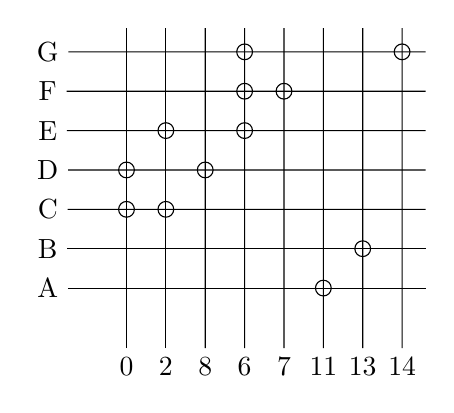
\begin{tikzpicture}
    \node (n0) at (0,0)            {0} ;
    \node (n1) at ($(n0)+(0.5,0)$) {2} ;
    \node (n2) at ($(n1)+(0.5,0)$) {8} ;
    \node (n3) at ($(n2)+(0.5,0)$) {6} ;
    \node (n4) at ($(n3)+(0.5,0)$) {7} ;
    \node (n5) at ($(n4)+(0.5,0)$) {11};
    \node (n6) at ($(n5)+(0.5,0)$) {13};
    \node (n7) at ($(n6)+(0.5,0)$) {14};

    \node (m0) at ($(n0)+(-1,1)$)   {A};
    \node (m1) at ($(m0)+ (0,0.5)$) {B};
    \node (m2) at ($(m1)+ (0,0.5)$) {C};
    \node (m3) at ($(m2)+ (0,0.5)$) {D};
    \node (m4) at ($(m3)+ (0,0.5)$) {E};
    \node (m5) at ($(m4)+ (0,0.5)$) {F};
    \node (m6) at ($(m5)+ (0,0.5)$) {G};

    \foreach \i in {0,1,2,3,4,5,6,7}
    {
        \draw (n\i) -- (0.5*\i,4+0.3);
    }

    \foreach \i in {0,1,2,3,4,5,6}
    {
        \draw (m\i) -- (3.5 + 0.3,\i*0.5+1);
    }

    % A
    \draw (2.5,1) circle (.1cm);

    % B
    \draw (3,1.5) circle (.1cm);

    % C
    \draw (0,2) circle (.1cm);
    \draw (0.5,2) circle (.1cm);

    % D
    \draw (0,2.5) circle (.1cm);
    \draw (1,2.5) circle (.1cm);

    % E
    \draw (0.5,3) circle (.1cm);
    \draw (1.5,3) circle (.1cm);

    % F
    \draw (1.5,3.5) circle (.1cm);
    \draw (2,3.5) circle (.1cm);

    % G
    \draw (1.5,4) circle (.1cm);
    \draw (3.5,4) circle (.1cm);
  \end{tikzpicture}
\end{center}

\newpage

Posso scegliere, per coprire il termine $2$, l'implicante C oppure l'implicante E. Scegliendo l'implicante E mi riconduco all'espressione della funzione trovata con la mappa di Karnaugh.
\begin{center}
  \begin{table}[h]
    \makegapedcells
    \centering
    {
      \begin{tabular}{|c|c|c|}
        \hline
        \textbf{Implicante} & \textbf{Termini implicati} & \textbf{Espressione} \\
        \hline
          A & 11 & $x \cdot \oline{y} \cdot z \cdot k$ \\
        \hline
          B & 13 & $x \cdot y \cdot \oline{z} \cdot k$ \\
        \hline
          G & 6,14 & $y \cdot z \cdot \oline{k}$ \\
        \hline
          F & 6,7 & $\oline{x} \cdot y \cdot z$ \\
        \hline
          D & 0,8 & $\oline{y} \cdot \oline{z} \cdot \oline{k}$ \\
        \hline
          E & 0,2 & $\oline{x} \cdot z \cdot \oline{k}$ \\
        \hline
      \end{tabular}
    }
  \end{table}
\end{center}

La funzione ottenuta è la seguente:
\begin{align*}
  \bm{f(x,y,z,k)} = \underbracket{(\oline{y} \cdot \oline{z} \cdot \oline{k})}_{\text{D}} + \underbracket{(x \cdot y \cdot \oline{z} \cdot k)}_{\text{B}} + \underbracket{(x \cdot \oline{y} \cdot z \cdot k)}_{\text{A}} + \underbracket{(\oline{x} \cdot y \cdot z)}_{\text{F}} + \underbracket{(\oline{x} \cdot z \cdot \oline{k})}_{\text{E}} + \underbracket{(y \cdot z \cdot \oline{k})}_{\text{G}}
\end{align*}

\newpage

\section{Schema logico}

\bigskip

\subsection*{Minterm:}

\begin{align*}
  \bm{f(x,y,z,k)} &= (\oline{x} \cdot \oline{y} \cdot \oline{z} \cdot \oline{k}) + (\oline{x} \cdot \oline{y} \cdot z \cdot \oline{k}) + (\oline{x} \cdot y \cdot z \cdot \oline{k}) + (\oline{x} \cdot y \cdot z \cdot k) + (x \cdot \oline{y} \cdot \oline{z} \cdot \oline{k}) + (x \cdot \oline{y} \cdot z \cdot k) + \\
  &\bigspace + (x \cdot y \cdot \oline{z} \cdot k) + (x \cdot y \cdot z \cdot \oline{k})
\end{align*}


% labels
\begin{textblock*}{10pt}(368pt,318pt)
  \scalebox{0.5}{$(\oline{x} \cdot \oline{y} \cdot \oline{z} \cdot \oline{k})$}
\end{textblock*}

\begin{textblock*}{10pt}(368pt,360pt)
  \scalebox{0.5}{$(\oline{x} \cdot \oline{y} \cdot z \cdot \oline{k})$}
\end{textblock*}

\begin{textblock*}{10pt}(368pt,403pt)
  \scalebox{0.5}{$(\oline{x} \cdot y \cdot z \cdot \oline{k})$}
\end{textblock*}

\begin{textblock*}{10pt}(368pt,446pt)
  \scalebox{0.5}{$(\oline{x} \cdot y \cdot z \cdot k)$}
\end{textblock*}

\begin{textblock*}{10pt}(368pt,488pt)
  \scalebox{0.5}{$(x \cdot \oline{y} \cdot \oline{z} \cdot \oline{k})$}
\end{textblock*}

\begin{textblock*}{10pt}(368pt,531pt)
  \scalebox{0.5}{$(x \cdot \oline{y} \cdot z \cdot k)$}
\end{textblock*}

\begin{textblock*}{10pt}(368pt,574pt)
  \scalebox{0.5}{$(x \cdot y \cdot \oline{z} \cdot k)$}
\end{textblock*}

\begin{textblock*}{10pt}(368pt,617pt)
  \scalebox{0.5}{$(x \cdot y \cdot z \cdot \oline{k})$}
\end{textblock*}

\begin{center}
  %minterm
  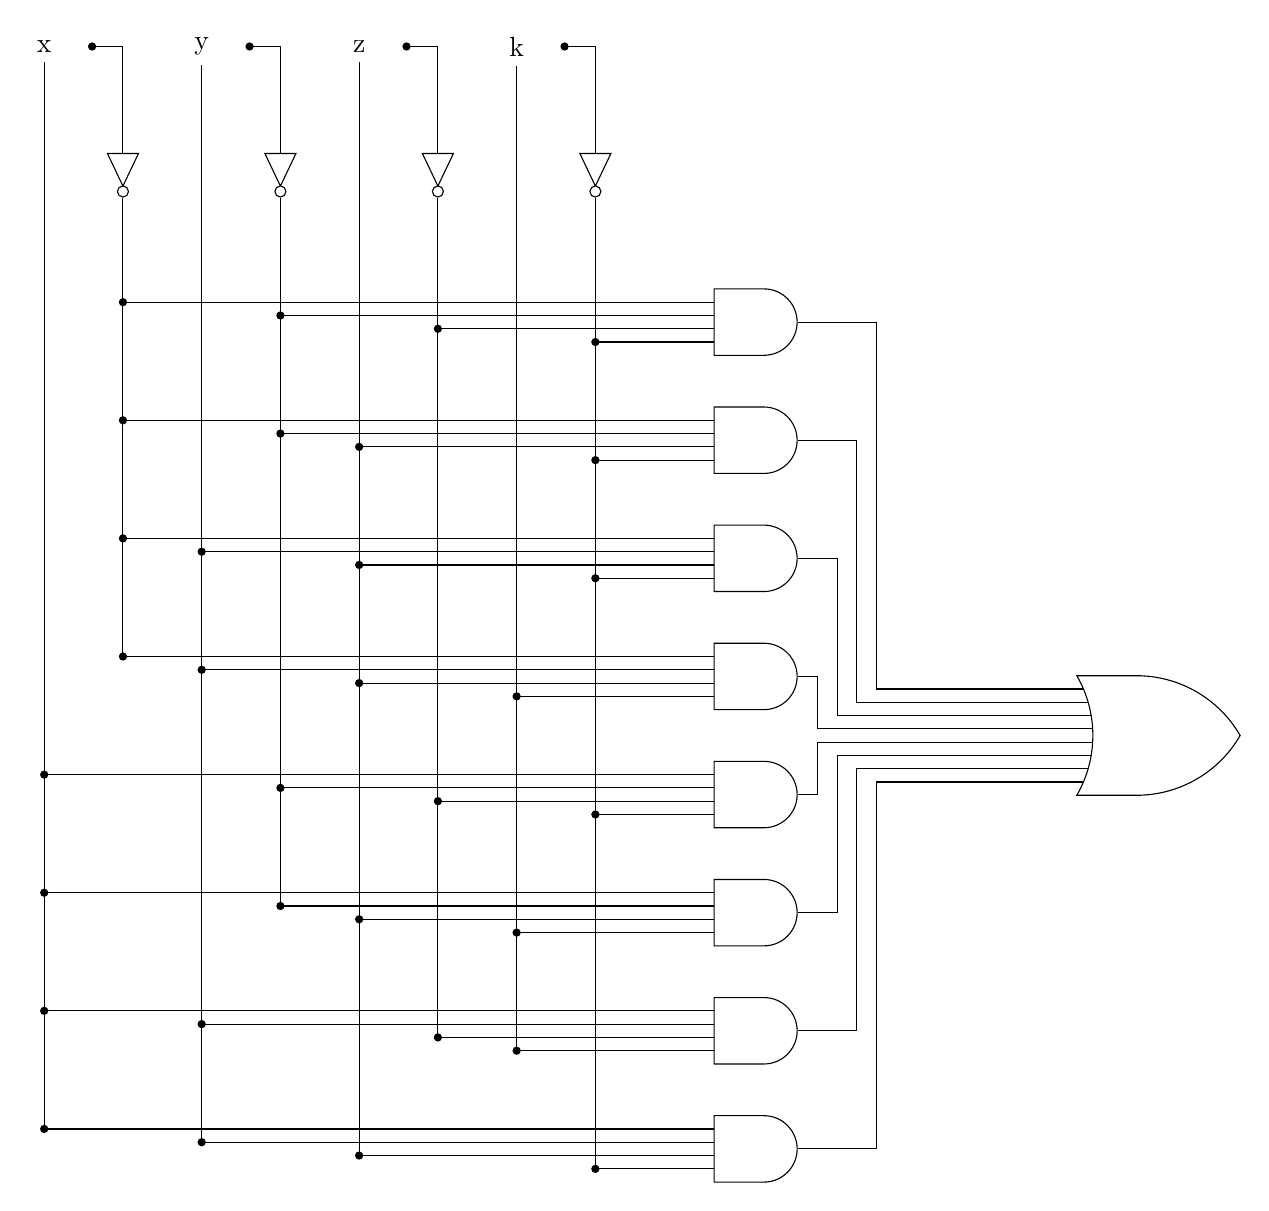
\begin{tikzpicture}
    \node (x0) at (0,0) {x};
    \node (x1) at ($(x0)+(2,0)$) {y};
    \node (x2) at ($(x1)+(2,0)$) {z};
    \node (x3) at ($(x2)+(2,0)$) {k};

    \node[not gate US, draw, rotate=-90] at ($(x0)+(1,-1.5)$) (Not0) {};
    \node[not gate US, draw, rotate=-90] at ($(x1)+(1,-1.5)$) (Not1) {};
    \node[not gate US, draw, rotate=-90] at ($(x2)+(1,-1.5)$) (Not2) {};
    \node[not gate US, draw, rotate=-90] at ($(x3)+(1,-1.5)$) (Not3) {};

    % connections with not ports
    \foreach \i in {0,1,2,3}
    {
        \path (x\i) -- coordinate (punt\i) (x\i -| Not\i.input);
        \draw (punt\i) node[branch] {} -| (Not\i.input);
    }

    \node[and gate US, draw, logic gate inputs=nnnn] at ($(x3)+(3,-3.5)$) (And0) {};
    \node[and gate US, draw, logic gate inputs=nnnn] at ($(And0)+(0,-1.5)$) (And1) {};
    \node[and gate US, draw, logic gate inputs=nnnn] at ($(And1)+(0,-1.5)$) (And2) {};
    \node[and gate US, draw, logic gate inputs=nnnn] at ($(And2)+(0,-1.5)$) (And3) {};
    \node[and gate US, draw, logic gate inputs=nnnn] at ($(And3)+(0,-1.5)$) (And4) {};
    \node[and gate US, draw, logic gate inputs=nnnn] at ($(And4)+(0,-1.5)$) (And5) {};
    \node[and gate US, draw, logic gate inputs=nnnn] at ($(And5)+(0,-1.5)$) (And6) {};
    \node[and gate US, draw, logic gate inputs=nnnn] at ($(And6)+(0,-1.5)$) (And7) {};

    \node[or gate US, draw, logic gate inputs=nnnnnnnn] at ($(And3)+(5,-0.75)$) (Or0) {};

    % minterm connections

    % 0
    \draw (Not0 |- And0.input 1) node[branch] {} -- (And0.input 1);
    \draw (Not1 |- And0.input 2) node[branch] {} -- (And0.input 2);
    \draw (Not2 |- And0.input 3) node[branch] {} -- (And0.input 3);
    \draw (Not3 |- And0.input 4) node[branch] {} -- (And0.input 4);

    % 1
    \draw (Not0 |- And1.input 1) node[branch] {} -- (And1.input 1);
    \draw (Not1 |- And1.input 2) node[branch] {} -- (And1.input 2);
    \draw (x2 |- And1.input 3) node[branch] {} -- (And1.input 3);
    \draw (Not3 |- And1.input 4) node[branch] {} -- (And1.input 4);

    % 2
    \draw (Not0 |- And2.input 1) node[branch] {} -- (And2.input 1);
    \draw (x1 |- And2.input 2) node[branch] {} -- (And2.input 2);
    \draw (x2 |- And2.input 3) node[branch] {} -- (And2.input 3);
    \draw (Not3 |- And2.input 4) node[branch] {} -- (And2.input 4);

    % 3
    \draw (Not0 |- And3.input 1) node[branch] {} -- (And3.input 1);
    \draw (x1 |- And3.input 2) node[branch] {} -- (And3.input 2);
    \draw (x2 |- And3.input 3) node[branch] {} -- (And3.input 3);
    \draw (x3 |- And3.input 4) node[branch] {} -- (And3.input 4);

    \draw (Not0) |- (And3.input 1);

    % 4
    \draw (x0 |- And4.input 1) node[branch] {} -- (And4.input 1);
    \draw (Not1 |- And4.input 2) node[branch] {} -- (And4.input 2);
    \draw (Not2 |- And4.input 3) node[branch] {} -- (And4.input 3);
    \draw (Not3 |- And4.input 4) node[branch] {} -- (And4.input 4);

    % 5
    \draw (x0 |- And5.input 1) node[branch] {} -- (And5.input 1);
    \draw (Not1 |- And5.input 2) node[branch] {} -- (And5.input 2);
    \draw (x2 |- And5.input 3) node[branch] {} -- (And5.input 3);
    \draw (x3 |- And5.input 4) node[branch] {} -- (And5.input 4);

    \draw (Not1) |- (And5.input 2);

    % 6
    \draw (x0 |- And6.input 1) node[branch] {} -- (And6.input 1);
    \draw (x1 |- And6.input 2) node[branch] {} -- (And6.input 2);
    \draw (Not2 |- And6.input 3) node[branch] {} -- (And6.input 3);
    \draw (x3 |- And6.input 4) node[branch] {} -- (And6.input 4);

    \draw (Not2) |- (And6.input 3);
    \draw (x3) |- (And6.input 4);

    % 7
    \draw (x0 |- And7.input 1) node[branch] {} -- (And7.input 1);
    \draw (x1 |- And7.input 2) node[branch] {} -- (And7.input 2);
    \draw (x2 |- And7.input 3) node[branch] {} -- (And7.input 3);
    \draw (Not3 |- And7.input 4) node[branch] {} -- (And7.input 4);

    \draw (x0) |- (And7.input 1);
    \draw (x1) |- (And7.input 2);
    \draw (x2) |- (And7.input 3);
    \draw (Not3) |- (And7.input 4);

    % AND to OR connection

    % 0
    \coordinate (p) at ($(And0.output)+(1,0)$);
    \draw (p) |- (Or0.input 1);
    \draw (And0.output) -- (p);

    %1
    \coordinate (p) at ($(And1.output)+(0.75,0)$);
    \draw (p) |- (Or0.input 2);
    \draw (And1.output) -- (p);

    %2
    \coordinate (p) at ($(And2.output)+(0.50,0)$);
    \draw (p) |- (Or0.input 3);
    \draw (And2.output) -- (p);

    %3
    \coordinate (p) at ($(And3.output)+(0.25,0)$);
    \draw (p) |- (Or0.input 4);
    \draw (And3.output) -- (p);

    %4
    \coordinate (p) at ($(And4.output)+(0.25,0)$);
    \draw (p) |- (Or0.input 5);
    \draw (And4.output) -- (p);

    %5
    \coordinate (p) at ($(And5.output)+(0.50,0)$);
    \draw (p) |- (Or0.input 6);
    \draw (And5.output) -- (p);

    %6
    \coordinate (p) at ($(And6.output)+(0.75,0)$);
    \draw (p) |- (Or0.input 7);
    \draw (And6.output) -- (p);

    %7
    \coordinate (p) at ($(And7.output)+(1,0)$);
    \draw (p) |- (Or0.input 8);
    \draw (And7.output) -- (p);
  \end{tikzpicture}
\end{center}

\newpage

\bigskip

\subsection*{Maxterm:}

\begin{align*}
  % line 1
  \bm{f(x,y,z,k)} &= (x+y+z+\oline{k}) \cdot (x+y+\oline{z}+\oline{k}) \cdot (x+\oline{y}+z+k) \cdot (x+\oline{y}+z+\oline{k}) \cdot (\oline{x}+y+z+\oline{k}) \cdot \\
  &\bigspace \cdot (\oline{x}+y+\oline{z}+k) \cdot (\oline{x}+\oline{y}+z+k) \cdot (\oline{x}+\oline{y}+\oline{z}+\oline{k})
\end{align*}

% labels
\begin{textblock*}{10pt}(366pt,282pt)
  \scalebox{0.5}{$(x + y + z + \oline{k})$}
\end{textblock*}

\begin{textblock*}{10pt}(366pt,324pt)
  \scalebox{0.5}{$(x + y + \oline{z} + \oline{k})$}
\end{textblock*}

\begin{textblock*}{10pt}(366pt,367pt)
  \scalebox{0.5}{$(x + \oline{y} + z + k)$}
\end{textblock*}

\begin{textblock*}{10pt}(366pt,410pt)
  \scalebox{0.5}{$(x + \oline{y} + z + \oline{k})$}
\end{textblock*}

\begin{textblock*}{10pt}(366pt,452pt)
  \scalebox{0.5}{$(\oline{x} + y + z + \oline{k})$}
\end{textblock*}

\begin{textblock*}{10pt}(366pt,495pt)
  \scalebox{0.5}{$(\oline{x} + y + \oline{z} + k)$}
\end{textblock*}

\begin{textblock*}{10pt}(366pt,538pt)
  \scalebox{0.5}{$(\oline{x} + \oline{y} + z + k)$}
\end{textblock*}

\begin{textblock*}{10pt}(366pt,581pt)
  \scalebox{0.5}{$(\oline{x} + \oline{y} + \oline{z} + \oline{k})$}
\end{textblock*}

\begin{center}
  \begin{tikzpicture}
    \node (x0) at (0,0) {x};
    \node (x1) at ($(x0)+(2,0)$) {y};
    \node (x2) at ($(x1)+(2,0)$) {z};
    \node (x3) at ($(x2)+(2,0)$) {k};

    \node[not gate US, draw, rotate=-90] at ($(x0)+(1,-1.5)$) (Not0) {};
    \node[not gate US, draw, rotate=-90] at ($(x1)+(1,-1.5)$) (Not1) {};
    \node[not gate US, draw, rotate=-90] at ($(x2)+(1,-1.5)$) (Not2) {};
    \node[not gate US, draw, rotate=-90] at ($(x3)+(1,-1.5)$) (Not3) {};

    % links with not ports
    \foreach \i in {0,1,2,3}
    {
        \path (x\i) -- coordinate (punt\i) (x\i -| Not\i.input);
        \draw (punt\i) node[branch] {} -| (Not\i.input);
    }

    \node[or gate US, draw, logic gate inputs=nnnn] at ($(x3)+(3,-3.5)$) (Or0) {};
    \node[or gate US, draw, logic gate inputs=nnnn] at ($(And0)+(0,-1.5)$) (Or1) {};
    \node[or gate US, draw, logic gate inputs=nnnn] at ($(And1)+(0,-1.5)$) (Or2) {};
    \node[or gate US, draw, logic gate inputs=nnnn] at ($(And2)+(0,-1.5)$) (Or3) {};
    \node[or gate US, draw, logic gate inputs=nnnn] at ($(And3)+(0,-1.5)$) (Or4) {};
    \node[or gate US, draw, logic gate inputs=nnnn] at ($(And4)+(0,-1.5)$) (Or5) {};
    \node[or gate US, draw, logic gate inputs=nnnn] at ($(And5)+(0,-1.5)$) (Or6) {};
    \node[or gate US, draw, logic gate inputs=nnnn] at ($(And6)+(0,-1.5)$) (Or7) {};

    \node[and gate US, draw, logic gate inputs=nnnnnnnn] at ($(Or3)+(5,-0.75)$) (And0) {};

    % maxterm connections
    % 0
    \draw (x0 |- Or0.input 1) node[branch] {} -- (Or0.input 1);
    \draw (x1 |- Or0.input 2) node[branch] {} -- (Or0.input 2);
    \draw (x2 |- Or0.input 3) node[branch] {} -- (Or0.input 3);
    \draw (Not3 |- Or0.input 4) node[branch] {} -- (Or0.input 4);

    % 1
    \draw (x0 |- Or1.input 1) node[branch] {} -- (Or1.input 1);
    \draw (x1 |- Or1.input 2) node[branch] {} -- (Or1.input 2);
    \draw (Not2 |- Or1.input 3) node[branch] {} -- (Or1.input 3);
    \draw (Not3 |- Or1.input 4) node[branch] {} -- (Or1.input 4);

    % 2
    \draw (x0 |- Or2.input 1) node[branch] {} -- (Or2.input 1);
    \draw (Not1 |- Or2.input 2) node[branch] {} -- (Or2.input 2);
    \draw (x2 |- Or2.input 3) node[branch] {} -- (Or2.input 3);
    \draw (x3 |- Or2.input 4) node[branch] {} -- (Or2.input 4);

    % 3
    \draw (x0 |- Or3.input 1) node[branch] {} -- (Or3.input 1);
    \draw (Not1 |- Or3.input 2) node[branch] {} -- (Or3.input 2);
    \draw (x2 |- Or3.input 3) node[branch] {} -- (Or3.input 3);
    \draw (Not3 |- Or3.input 4) node[branch] {} -- (Or3.input 4);

    \draw (x0) |- (Or3.input 1);

    % 4
    \draw (Not0 |- Or4.input 1) node[branch] {} -- (Or4.input 1);
    \draw (x1 |- Or4.input 2) node[branch] {} -- (Or4.input 2);
    \draw (x2 |- Or4.input 3) node[branch] {} -- (Or4.input 3);
    \draw (Not3 |- Or4.input 4) node[branch] {} -- (Or4.input 4);

    % 5
    \draw (Not0 |- Or5.input 1) node[branch] {} -- (Or5.input 1);
    \draw (x1 |- Or5.input 2) node[branch] {} -- (Or5.input 2);
    \draw (Not2 |- Or5.input 3) node[branch] {} -- (Or5.input 3);
    \draw (x3 |- Or5.input 4) node[branch] {} -- (Or5.input 4);

    \draw (x1) |- (Or5.input 2);

    % 6
    \draw (Not0 |- Or6.input 1) node[branch] {} -- (Or6.input 1);
    \draw (Not1 |- Or6.input 2) node[branch] {} -- (Or6.input 2);
    \draw (x2 |- Or6.input 3) node[branch] {} -- (Or6.input 3);
    \draw (x3 |- Or6.input 4) node[branch] {} -- (Or6.input 4);

    \draw (x2) |- (Or6.input 3);
    \draw (x3) |- (Or6.input 4);

    % 7
    \draw (Not0 |- Or7.input 1) node[branch] {} -- (Or7.input 1);
    \draw (Not1 |- Or7.input 2) node[branch] {} -- (Or7.input 2);
    \draw (Not2 |- Or7.input 3) node[branch] {} -- (Or7.input 3);
    \draw (Not3 |- Or7.input 4) node[branch] {} -- (Or7.input 4);

    \draw (Not0) |- (Or7.input 1);
    \draw (Not1) |- (Or7.input 2);
    \draw (Not2) |- (Or7.input 3);
    \draw (Not3) |- (Or7.input 4);

    % OR to AND connection

    % 0
    \coordinate (p) at ($(Or0.output)+(1,0)$);
    \draw (p) |- (And0.input 1);
    \draw (Or0.output) -- (p);

    %1
    \coordinate (p) at ($(Or1.output)+(0.75,0)$);
    \draw (p) |- (And0.input 2);
    \draw (Or1.output) -- (p);

    %2
    \coordinate (p) at ($(Or2.output)+(0.50,0)$);
    \draw (p) |- (And0.input 3);
    \draw (Or2.output) -- (p);

    %3
    \coordinate (p) at ($(Or3.output)+(0.25,0)$);
    \draw (p) |- (And0.input 4);
    \draw (Or3.output) -- (p);

    %4
    \coordinate (p) at ($(Or4.output)+(0.25,0)$);
    \draw (p) |- (And0.input 5);
    \draw (Or4.output) -- (p);

    %5
    \coordinate (p) at ($(Or5.output)+(0.50,0)$);
    \draw (p) |- (And0.input 6);
    \draw (Or5.output) -- (p);

    %6
    \coordinate (p) at ($(Or6.output)+(0.75,0)$);
    \draw (p) |- (And0.input 7);
    \draw (Or6.output) -- (p);

    %7
    \coordinate (p) at ($(Or7.output)+(1,0)$);
    \draw (p) |- (And0.input 8);
    \draw (Or7.output) -- (p);
  \end{tikzpicture}
\end{center}

\newpage

\bigskip

\subsection*{Funzione semplificata:}
\begin{align*}
  \bm{f(x,y,z,k)} = (\oline{y} \cdot \oline{z} \cdot \oline{k}) + (x \cdot y \cdot \oline{z} \cdot k) + (x \cdot \oline{y} \cdot z \cdot k) + (\oline{x} \cdot y \cdot z) + (\oline{x} \cdot z \cdot \oline{k}) + (y \cdot z \cdot \oline{k})
\end{align*}

\bigskip

\bigskip

\bigskip

% labels
\begin{textblock*}{10pt}(368pt,311pt)
  \scalebox{0.5}{$(x \cdot y \cdot \oline{z} \cdot k)$}
\end{textblock*}

\begin{textblock*}{10pt}(368pt,353pt)
  \scalebox{0.5}{$(x \cdot \oline{y} \cdot z \cdot k)$}
\end{textblock*}

\begin{textblock*}{10pt}(371pt,398pt)
  \scalebox{0.5}{$(\oline{y} \cdot \oline{z} \cdot \oline{k})$}
\end{textblock*}

\begin{textblock*}{10pt}(371pt,441pt)
  \scalebox{0.5}{$(\oline{x} \cdot y \cdot z)$}
\end{textblock*}

\begin{textblock*}{10pt}(371pt,483pt)
  \scalebox{0.5}{$(\oline{x} \cdot \cdot z \cdot \oline{k})$}
\end{textblock*}

\begin{textblock*}{10pt}(371pt,526pt)
  \scalebox{0.5}{$(y \cdot z \cdot \oline{k})$}
\end{textblock*}

\begin{center}
  \begin{tikzpicture}
    \node (x0) at (0,0) {x};
    \node (x1) at ($(x0)+(2,0)$) {y};
    \node (x2) at ($(x1)+(2,0)$) {z};
    \node (x3) at ($(x2)+(2,0)$) {k};

    \node[not gate US, draw, rotate=-90] at ($(x0)+(1,-1.5)$) (Not0) {};
    \node[not gate US, draw, rotate=-90] at ($(x1)+(1,-1.5)$) (Not1) {};
    \node[not gate US, draw, rotate=-90] at ($(x2)+(1,-1.5)$) (Not2) {};
    \node[not gate US, draw, rotate=-90] at ($(x3)+(1,-1.5)$) (Not3) {};

    % connections with not ports
    \foreach \i in {0,1,2,3}
    {
        \path (x\i) -- coordinate (punt\i) (x\i -| Not\i.input);
        \draw (punt\i) node[branch] {} -| (Not\i.input);
    }

    \node[and gate US, draw, logic gate inputs=nnnn] at ($(x3)+(3,-3.5)$) (And0) {};
    \node[and gate US, draw, logic gate inputs=nnnn] at ($(And0)+(0,-1.5)$) (And1) {};
    \node[and gate US, draw, logic gate inputs=nnn]  at ($(And1)+(0,-1.5)$) (And2) {};
    \node[and gate US, draw, logic gate inputs=nnn]  at ($(And2)+(0,-1.5)$) (And3) {};
    \node[and gate US, draw, logic gate inputs=nnn]  at ($(And3)+(0,-1.5)$) (And4) {};
    \node[and gate US, draw, logic gate inputs=nnn]  at ($(And4)+(0,-1.5)$) (And5) {};

    \node[or gate US, draw, logic gate inputs=nnnnnn] at ($(And3)+(5,0.75)$) (Or0) {};

    % connections

    % 0
    \draw (x0 |- And0.input 1) node[branch] {} -- (And0.input 1);
    \draw (x1 |- And0.input 2) node[branch] {} -- (And0.input 2);
    \draw (Not2 |- And0.input 3) node[branch] {} -- (And0.input 3);
    \draw (x3 |- And0.input 4) node[branch] {} -- (And0.input 4);

    % 1
    \draw (x0 |- And1.input 1) node[branch] {} -- (And1.input 1);
    \draw (Not1 |- And1.input 2) node[branch] {} -- (And1.input 2);
    \draw (x2 |- And1.input 3) node[branch] {} -- (And1.input 3);
    \draw (x3 |- And1.input 4) node[branch] {} -- (And1.input 4);

    \draw (x0) |- (And1.input 1);
    \draw (x3) |- (And1.input 4);

    % 2
    \draw (Not1 |- And2.input 1) node[branch] {} -- (And2.input 1);
    \draw (Not2 |- And2.input 2) node[branch] {} -- (And2.input 2);
    \draw (Not3 |- And2.input 3) node[branch] {} -- (And2.input 3);

    \draw (Not1) |- (And2.input 1);
    \draw (Not2) |- (And2.input 2);

    % 3
    \draw (Not0 |- And3.input 1) node[branch] {} -- (And3.input 1);
    \draw (x1 |- And3.input 2) node[branch] {} -- (And3.input 2);
    \draw (x2 |- And3.input 3) node[branch] {} -- (And3.input 3);

    % 4
    \draw (Not0 |- And4.input 1) node[branch] {} -- (And4.input 1);
    \draw (x2 |- And4.input 2) node[branch] {} -- (And4.input 2);
    \draw (Not3 |- And4.input 3) node[branch] {} -- (And4.input 3);

    \draw (Not0) |- (And4.input 1);

    % 5
    \draw (x1 |- And5.input 1) node[branch] {} -- (And5.input 1);
    \draw (x2 |- And5.input 2) node[branch] {} -- (And5.input 2);
    \draw (Not3 |- And5.input 3) node[branch] {} -- (And5.input 3);

    \draw (x1) |- (And5.input 1);
    \draw (x2) |- (And5.input 2);
    \draw (Not3) |- (And5.input 3);

    % AND to OR connection

    % 0
    \coordinate (p) at ($(And0.output)+(0.9,0)$);
    \draw (p) |- (Or0.input 1);
    \draw (And0.output) -- (p);

    %1
    \coordinate (p) at ($(And1.output)+(0.65,0)$);
    \draw (p) |- (Or0.input 2);
    \draw (And1.output) -- (p);

    %2
    \coordinate (p) at ($(And2.output)+(0.50,0)$);
    \draw (p) |- (Or0.input 3);
    \draw (And2.output) -- (p);

    %3
    \coordinate (p) at ($(And3.output)+(0.50,0)$);
    \draw (p) |- (Or0.input 4);
    \draw (And3.output) -- (p);

    %4
    \coordinate (p) at ($(And4.output)+(0.75,0)$);
    \draw (p) |- (Or0.input 5);
    \draw (And4.output) -- (p);

    %5
    \coordinate (p) at ($(And5.output)+(1,0)$);
    \draw (p) |- (Or0.input 6);
    \draw (And5.output) -- (p);
  \end{tikzpicture}
\end{center}

\end{document}
